\chapter{化学键和分子结构}\label{chp:chemkey}
我们已经学习了原子结构以及原子结构与元素性质递变关系的初步知识，从本章起，我们将学习有关原子怎样互相结合，以及分子结构与物质性质的关系等初步知识。

\section{离子键}
\subsection{什么是化学键}
人们已经发现和合成了几百万种物质。
为什么仅仅一百零几种元素的原子能够形成这么多种形形色色的物质呢？ 原子是怎样互相结合的？
为什么两个氢原子能自动结合成氢分子，而两个氦原子不能结合在一起？ 为什么原子间按一定数目比互相结合？
原子结合成分子后，性质为什么与原来的差别很大？
为了弄清以上的许多问题，首先，就要在原子结构知识基础上，进一步研究原子在形成分子时的相互作用。

原子既然可以结合成分子，原子之间必然存在着相互作用，这种相互作用不仅存在于直接相邻的原子之间，而且也存在于分子内的非直接相邻的原子之间。
前一种相互作用比较强烈，是使原子相互作用而联结成分子的主要因素，破坏它要消耗比较大的能量。
这种相邻的两个或多个原子之间强烈的相互作用，通常叫做\Concept{化学键}。

化学键的主要类型有离子键、共价键、金属键等，在这一章里，我们先学习离子键和共价键。

\subsubsection{离子键}
我们已经知道，金属钠跟氯气能发生反应，生成氯化钠：
\[ \ce{ 2Na + Cl2 \xlongequal{\quad} 2NaCl }\]

因为钠原子的电离能很小，容易失去电子，而氯原子很容易结合电子。
当钠跟氯气起反应时，钠原子的 $3s$ 电子转移到氯原子的 $3p$ 轨道上：
\begin{figurehere}
  \includegraphics{1-a.pdf}
\end{figurehere}

钠原子失去 1 个 $3s$ 电子，形成类似氖原子的稳定电子层结构，带上一个单位正电荷，成为钠离子（\ce{Na+}）；氯原子得到 1 个电子，形成类似氩原子的稳定电子层结构，带上一个单位负电荷，成为氯离子（\ce{Cl-}）。
\begin{figurehere}
  \includegraphics{1-b.pdf}
\end{figurehere}

钠离子和氯离子之间除了有静电相互吸引作用外，还有电子与电子、原子核与原子核之间的相互排斥作用。
当两种离子接近到某一定距离时，吸引和排斥作用达到了平衡，于是阴、阳离子之间就形成了稳定的化学键。

氯化钠的生成也可以用电子式来表示：
\[ \electformular{Na}{n}{n}{n}{n}{x}{n}{n}{n} + \electformular{Cl}{d}{n}{d}{d}{d}{d}{d}{d} \ce{->} \ce{Na+}\Bigl[\electformular{Cl}{x}{d}{d}{d}{d}{d}{d}{d}\Bigr]^-\]

象氯化钠那样，\emph{阴、阳离子间通过静电作用所形成的化学键}叫做\Concept{离子键}。

活泼金属（如钾、钠、钙等）跟活泼非金属（如氯、溴等）化合时，都能形成离子键。例如，溴化钙就是由离子键所形成的。
\[\electformular{Ca}{n}{n}{n}{n}{x}{x}{n}{n} + 2\,\electformular{Br}{d}{n}{d}{d}{d}{d}{d}{d} \ce{->} \Bigl[\electformular{Br}{d}{d}{d}{d}{d}{x}{d}{d}\Bigr]^-\ce{Ca^2+}\Bigl[\electformular{Br}{x}{d}{d}{d}{d}{d}{d}{d}\Bigr]^-\]

\subsection{离子的结构特征}
\subsubsection{离子的电荷}
离子是带电荷的原子或原子团，离子所带电荷的符号和数目与原子成键时得失电子数有关。
例如，镁跟氯起反应生成氯化镁，每个镁原子失去 2 个电子形成 \ce{Mg^2+}，每个氯原子得到 1 个电子形成 \ce{Cl-}。

\subsubsection{离子的电子层结构}
主族元素所形成的离子的电子层一般是饱和的，例如，\ce{Li+}、\ce{Be^2+} 等离子最外层是两个电子，\ce{Na+}、\ce{K+}、\ce{Ca^2+}、\ce{Mg^2+}、\ce{Al^3+}、\ce{O^2-}、\ce{S^2-}、\ce{F-}、\ce{Cl-} 等离子最外层是 8 个电子; 副族和第 \MyRoman{8} 族元素所形成的离子的电子层常常是不饱和的，例如，\ce{Fe^3+} 最外层有 13 个电子，\ce{Co^3+} 最外层有 14 个电子，等等。

\subsubsection{离子的半径}
由于阳离子是由原子失去外层电子而形成的，所以，阳离子的半径比相应的原子半径小，例如：

\begin{tblr}{colspec={l*5{c}},hlines=0pt,vlines=0pt}
  & \ce{Li} & \ce{Na} & \ce{K} & \ce{Rb} & \ce{Cs} \\
  原子半径（\qty{e-10}{m}）& 1.52 & 1.86 & 2.27 & 2.48 & 2.65 \\
  离子半径（\qty{e-10}{m}）& 0.68 & 0.97 & 1.33 & 1.47 & 1.67 \\
\end{tblr}

由于阴离子的外层电子数比相应的原子增多，而核电荷没有变化，所以，阴离子的半径比相应的原子半径大。例如：

\begin{tblr}{colspec={l*4{c}},hlines=0pt,vlines=0pt}
  & \ce{F} & \ce{Cl} & \ce{Br} & \ce{I}  \\
  原子半径（\qty{e-10}{m}）& 0.71 & 0.99 & 1.14 & 1.33 \\
  离子半径（\qty{e-10}{m}）& 1.33 & 1.81 & 1.96 & 2.20 \\
\end{tblr}

对于电子层结构相同的离子，如 \ce{F-}、\ce{Na+}、\ce{Mg^2+}、\ce{Al^3+}（它们的电子层结构与氖原子相同），随着核电荷的逐渐增加，离子半径逐渐减小。
下面列出这几种离子的半径（\qty{e-10}{m}）。

\mbox{}\hfill\begin{tblr}{colspec={*4{c}},hlines=0pt,vlines=0pt}
   \ce{F-} & \ce{Na+} & \ce{Mg^2+} & \ce{Al^3+} \\
   1.33 & 0.97 & 0.65 & 0.50 \\
\end{tblr}\hfill\mbox{}

\subsection{离子晶体}
以离子键结合的化合物就是离子化合物。
离子化合物在室温下是以晶体形式存在。
离子间通过离子键结合而成的品体叫做\Concept{离子晶体}。

在离子晶体中，阴、阳离子按一定规律在空间排列。
\cref{fig:1-1} 所示是 \ce{NaCl} 的晶体结构，\cref{fig:1-2} 所示是 \ce{CsCl} 的晶体结构。
\begin{figure}
  \begin{minipage}[b]{0.38\linewidth}\centering
    \includegraphics{1-1.pdf}
    \caption{\ce{NaCl} 的晶体结构}\label{fig:1-1}
  \end{minipage}
  \begin{minipage}[b]{0.58\linewidth}\centering
    \includegraphics{1-2.pdf}
    \caption{\ce{CsCl} 的晶体结构}\label{fig:1-2}
  \end{minipage}
\end{figure}

在 \ce{NaCl} 晶体中，每个 \ce{Na+} 离子同时吸引着 6 个 \ce{Cl-} 离子，每个 \ce{Cl-} 离子也同时吸引着 6 个 \ce{Na+} 离子。
在 \ce{CsCl} 晶体中，每个 \ce{Cs+} 离子同时吸引着 8 个 \ce{Cl-} 离子，每个 \ce{Cl-} 离子也同时吸引着 8 个 \ce{Cs+} 离子。
因此，在 \ce{NaCl} 或 \ce{CsCl} 晶体中都不存在着单个的 \ce{NaCl} 分子或单个的 \ce{CsCl} 分子。
但是，在这两种晶体里，阴、阳离子数目的比都是 $1:1$。
所以，严格地说，\ce{NaCl} 和 \ce{CsCl} 都是表示离子晶体中离子的个数比，它们都是用元素符号表示物质组成的化学式，而不是表示分子组成的分子式\footnote{重排注：分子式不是一个准确的表达，现中学教材都已改使用化学式这个概念。本套教材其余部分均已相应修改，这里因句意表达的需要，沿用原书的表达方式。}。

在离子化合物中，离子间存在着较强的离子键，因此，离子化合物一般说来，硬度较高，密度较大，难于压缩，难于挥发，有较高的熔点和沸点。

\begin{Practice}[习题]
\begin{question}
  \item 用轨道表示式画出 \ce{Mg} 和 \ce{F} 原子的电子层和亚层的结构，并用电子式来表示 \ce{MgF2} 离子键的形成过程。
  \item 用轨道表示式画出 \ce{Na} 和 \ce{S} 原子的电子层和亚层的结构，并用电子式来表示 \ce{Na2S} 离子键的形成过程。
  \item 用轨道表示式画出 \ce{Ba^2+}、\ce{Ag+}、\ce{Al^3+}、\ce{Fe^2+}、\ce{Fe^3+} 的离子的电子层和亚层的结构。
  \item 为什么说离子晶体中不存在单个的分子？
\end{question}
\end{Practice}

\section{共价键}
\subsection{共价键}
共价键是一种重要类型的化学键。
现在举几种单质和化合物为例来说明共价键的形成和性质。

首先，我们来学习氢原子是怎样结合成氢分子的。
在通常状况下，当一个氢原子和另一个氢原子接近时，就相互作用而生成氢分子。
\[ \ce{ H + H = H2}\]

在形成氢分子过程中，电子不是从一个氢原子转移到另一个氢原子，而是在两个氢原子间共用。
这两个共用的电子，填充了两个氢原子的 $1s$ 轨道，在两个原子核周围运动。
这样,每个氢原子的 $1s$ 轨道是充满的，每个氢原子具有氦原子的稳定结构。

氢分子中的共用电子对可用下式表示：
\begin{figurehere}
  \includegraphics{1-c.pdf}
\end{figurehere}

氢分子的电子式为：\electformular{H}{n}{n}{n}{n}{d}{x}{n}{n}\:\!\ce{H}。

在化学上常用一根短线表示一对共用电子，因此，氢分子又可表示为: \ce{H-H}。

从氢分子的电子云分布来看，当两个电子自旋方向相同的氢原子互相接近时，两个核间的电子云是稀疏的，不能形成稳定的氢分子; 当两个电子自旋方向相反的氢原子互相接近时，两个核间的电子云密集，对两核产生引力，能形成稳定的 \ce{H2} 分子（\cref{fig:1-3}）。
\begin{figure}
  \includegraphics{1-3.pdf}
  \caption{氢分子的形成}\label{fig:1-3}
\end{figure}

氢分子的形成过程也可以用电子云的重叠来说明，两个原子的电子云部分重叠以后，两核间的电子云密集，形成稳定分子。
电子云重叠愈多，分子愈稳定。



\par\medskip\noindent
\begin{minipage}{0.5\linewidth}\parindent2em
象氢分子那样，\emph{原子间通过共用电子对（电子云重叠）所形成的化学键，叫做}\Concept{共价键}。

在分子中，两个成键的原子的核间的平均距离叫做\Concept{键长}。
例如，\ce{H-H} 键长 \qty{0.74e-10}{m}（\cref{fig:1-4}），\ce{C-C} 键长 \qty{1.54e-10}{m}，\ce{Cl-Cl} 键长 \qty{1.98e-10}{m}。
一般说来，两个原子之间所形成的键越短的，键就越强，越牢固。
\end{minipage}\hfill
\begin{minipage}{0.45\linewidth}
\begin{figurehere}
  \includegraphics{1-4.pdf}
  \caption{\ce{H-H} 键的键长}\label{fig:1-4}
\end{figurehere}
\end{minipage}
\par\medskip

在 \ce{H} 原子形成 \ce{H2} 的过程中,要放出热量：
\[ \ce{ H + H  -> H2} + \qty{104.2}{kCal} \]

由上式可知，\qty{1}{mol} \ce{H} 原子和 \qty{1}{mol} 摩尔 \ce{H} 原子作用，生成 \qty{1}{mol} \ce{H2} 分子，放出 \qty{104.2}{kCal} 热。
上式也可说明 \ce{H2} 分子比 \ce{H} 原子的能量降低，\ce{H2} 分子比 \ce{H} 原子稳定。

如果要使 \qty{1}{mol} \ce{H2} 分子分裂为 \qty{2}{mol} \ce{H} 原子，同样也需要吸收 \qty{104.2}{kCal} 的热：
\[ \ce{H2} + \qty{104.2}{kCal} \ce{-> H + H }\]

由上式可知，要拆开 \qty{1}{mol} \ce{H-H} 键，需要吸收 \qty{104.2}{kCal} 的能量，这个能量就是 \ce{H-H} 键的\Concept{键能}。
键能越大，表示化学键越牢固，含有该键的分子越稳定。

\cref{tab:1-1} 列出了某些共价键的键能的数值。
\begin{table}
  \caption{某些共价键的键能（\unit{kCal/mol}）}\label{tab:1-1}
  \begin{tblr}{colspec={X[c]X[r]*3{cr}X[c]X[r]},hline{2}=0.8pt,vline{3,5,7,9}=1.5pt,row{1}={m,c}}
    键 & 键能 & 键 & 键能 & 键 & 键能 & 键 & 键能 & 键 & 键能\\
    \ce{H-H}   & 104.2  & \ce{Cl-Cl} & 58.0   & \ce{Br-Br} & 46.3  & \ce{I-I}   & 36.5  & \ce{C-C}   & 83.1 \\
    \ce{C-H}   & 98.8   & \ce{O-H}   & 110.6  & \ce{N-H}   & 93.4   & \ce{H-Cl}  & 103.2   & \ce{H-I}   & 71.4 \\
  \end{tblr}
\end{table}

\begin{Theorem}{讨论}
  现有反应
  \[ \ce{ H2 + Cl2 \xlongequal{\quad} 2HCl } + \qty{44.2}{kCal}\]
  试讨论反应物（\ce{H-H}、\ce{Cl-Cl}）和生成物（\ce{H-Cl}）的键能与这个反应的反应热的关系。
\end{Theorem}

双原子的 \ce{Cl2} 分子的形成跟 \ce{H2} 分子相似。两个氯原子共用一对电子，这一对电子互相充填未充满的 $3p$ 轨道，这样，每个氯原子具有氩原子的电子层结构。
\begin{figurehere}
  \includegraphics{1-d.pdf}
\end{figurehere}

氯分子可以用下列式子表示：
\[ \electformular{Cl}{x}{x}{x}{x}{d}{x}{x}{x}\:\!\electformular{Cl}{n}{n}{d}{d}{d}{d}{d}{d} \qquad\ce{Cl-Cl} \]

氮分子的形成跟氯分子相似，只是有三对 $p$ 电子共用，形成三键。
\begin{figurehere}
  \includegraphics{1-e.pdf}
\end{figurehere}

氮分子可以用下列式子表示：
\[ \electformularr{N}{x}{x}{x}{x}{x}\:\electformularl{N}{d}{d}{d}{d}{d}\qquad \ce{N#N} \]

现在举两个不同原子以共价键结合成分子的例子，如 \ce{HCl} 分子：
\begin{figurehere}
  \includegraphics{1-f.pdf}
\end{figurehere}

\ce{HCl} 分子可用下列式子表示：
\[\ce{H}\,\electformular{Cl}{x}{d}{d}{d}{d}{d}{d}{d}
\qquad\qquad\qquad\ce{H-Cl} \]

再如 \ce{H2O} 分子：
\begin{figurehere}
  \includegraphics{1-g.pdf}
\end{figurehere}

\ce{H2O} 分子可用下式表示：
\[
\begin{tikzpicture}[baseline=(h2.base),inner sep=2.5pt]
  \node (o) at (0,0){\ce{O}};
  \node (h1) at (-1.2em,0){\ce{H}};
  \node (h2) at (0,-1.2em){\ce{H}};
  \pic at ([yshift=-0.4ex]o.west){x}; 
  \pic at ([yshift= 0.4ex]o.west){d}; 
  \pic at ([xshift=-0.4ex]o.north){d}; 
  \pic at ([xshift= 0.4ex]o.north){d}; 
  \pic at ([yshift= 0.4ex]o.east){d}; 
  \pic at ([yshift=-0.4ex]o.east){d}; 
  \pic at ([xshift= 0.4ex]o.south){d}; 
  \pic at ([xshift=-0.4ex]o.south){x};
\end{tikzpicture} 
\qquad\qquad\qquad\chemfig{H-[:37.5]O-[:-37.5]H}
\]

\subsection{共价键的饱和性和方向性}
根据上面学过的几种单质和化合物中共价键的形成的知识，我们可以看出共价键具有以下两个共同的性质。

\subsubsection{饱和性}
由于一个原子的未成对电子跟另一个原子的自旋相反的电子配对成键后，就不能跟第三个电子配对成键，因此，一个原子有几个未成对电子，就可和几个自旋相反的电子配对成键。
这就是共价键的饱和性。
例如，硫原子和氢原子能结合生成硫化氢分子，因为每个硫原子有两个未成对的 $3p$ 电子，每个氢原子有一个未成对的 $1s$ 电子，所以，一个硫原子可以跟两个氢原子结合成 \ce{H2S} 分子，而不可能生成 \ce{H3S} 或 \ce{H4S} 的分子。

\subsubsection{方向性}
\par\medskip\noindent
\begin{minipage}{0.63\linewidth}\parindent2em
我们知道,除 $s$ 轨道的电子云是球形对称的以外，其它轨道（$p$ 轨道、 $d$ 轨道等）的电子云都具有一定的伸展方向。
在形成共价键时，成键电子的电子云重叠愈多，核间电子云密度愈大，形成的共价键愈稳固。
因此，共价键的形成尽可能沿着电子云密度最大的方向。
例如，在硫原子跟氢原子结合生成 \ce{H2S} 分子时，因为硫原子的最外层两个不成对的 $3p$ 电子的电子云互成直角，氢原子的 $1s$ 电子云要沿着直角的方向跟 $3p$ 电子云重叠，这样 \ce{H2S} 分子中两个共价键的夹角应接近 \ang{90}（\cref{fig:1-5}）。
\end{minipage}\hfill
\begin{minipage}{0.35\linewidth}
\begin{figurehere}
  \includegraphics{1-5.pdf}
  \caption{硫化氢分子的成键}\label{fig:1-5}
\end{figurehere}
\end{minipage}
\par\medskip

在分子中键和键之间的夹角叫做\Concept{键角}。
例如，水分子中两个 \ce{O-H} 键间的夹角是 \ang{104.5}，二氧化碳分子中两个 \ce{C=O} 键成直线，夹角是 \ang{180}，氨分子中两个 \ce{N-H} 键间的夹角是 \ang{107;18;}，甲烷分子中两个 \ce{C-H} 键间的夹角是 \ang{109;28;}。

\subsection{配位键}
上面介绍的共价键中，电子对都是由两个原子各提供未成对电子而形成的。
还有一类特殊的共价键，电子对是由一个原子单方面提供而跟另一个原子共用的。
这样的共价键叫做\Concept{配位键}。

现在以铵离子 \ce{NH4+} 为例来说明配位键的形成。
我们已经知道，氨跟酸起反应生成铵盐，例如：
\[ \ce{ NH3 + HCl \xlongequal{\quad} NH4Cl }\]

这个反应可用离子方程式来表示：
\[ \ce{ NH3 + H+ = NH4+}\]

上式表示氨跟能产生氢离子的物质（酸）相作用，生成铵离子。

氨分子的电子式是
\[\begin{tikzpicture}[baseline=(n.base),inner sep=2.5pt]
  \node (n){N};
  \foreach \x in {1,2,3}
  {
    \node(h\x) at (90*\x:1.2em) {H};
  }
  \pic at ([yshift=-0.4ex]n.west){d}; 
  \pic at ([yshift= 0.4ex]n.west){d}; 
  \pic at ([xshift=-0.4ex]n.north){d}; 
  \pic at ([xshift= 0.4ex]n.north){d}; 
  \pic at ([yshift= 0.4ex]n.east){d}; 
  \pic at ([yshift=-0.4ex]n.east){d}; 
  \pic at ([xshift= 0.4ex]n.south){d}; 
  \pic at ([xshift=-0.4ex]n.south){d};
\end{tikzpicture}\]
氮原子上有一对没有跟其它原子共用的电子（孤对电子）。氢离子（\ce{H+}）是氢原子失去 $1s$ 电子而形成的，它具有一个 $1s$ 空轨道。
当氨分子跟氢离子相作用时，氨分子上的孤对电子进入氢离子的空轨道，这一对电子在氮、氢原子间共用，形成了配位键。
配位键可以用 \ce{A\to B} 来表示，其中 \ce{A} 是提供孤对电子的原子，\ce{B} 是具有空轨道接受电子的原子。
\[
\begin{tikzpicture}[baseline=(N.base),inner sep=2.5pt]
  \node (N) {\ce{N}};
  \foreach \x in {1,2,3}
  {
    \node(h\x) at (90*\x:1.2em) {H};
  }
  \pic at ([yshift=-0.4ex]N.west){d}; 
  \pic at ([yshift= 0.4ex]N.west){d}; 
  \pic at ([xshift=-0.4ex]N.north){d}; 
  \pic at ([xshift= 0.4ex]N.north){d}; 
  \pic at ([yshift= 0.4ex]N.east){d}; 
  \pic at ([yshift=-0.4ex]N.east){d}; 
  \pic at ([xshift= 0.4ex]N.south){d}; 
  \pic at ([xshift=-0.4ex]N.south){d};
\end{tikzpicture}
\,+\, \ce{H+ -> }
\left[
\begin{tikzpicture}[baseline=(N.base),inner sep=2.5pt]
  \node (N) {\ce{N}};
  \foreach \x in {1,2,3,4}
  {
    \node(h\x) at (90*\x:1.2em) {H};
  }
  \pic at ([yshift=-0.4ex]N.west){d}; 
  \pic at ([yshift= 0.4ex]N.west){d}; 
  \pic at ([xshift=-0.4ex]N.north){d}; 
  \pic at ([xshift= 0.4ex]N.north){d}; 
  \pic at ([yshift= 0.4ex]N.east){d}; 
  \pic at ([yshift=-0.4ex]N.east){d}; 
  \pic at ([xshift= 0.4ex]N.south){d}; 
  \pic at ([xshift=-0.4ex]N.south){d};
\end{tikzpicture}
\right]^+\ \text{或}\ 
\left[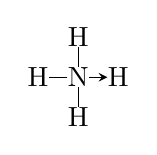
\begin{tikzpicture}[baseline=(N.base),inner sep=0pt]
  \node (N) {\ce{N}};
  \node (h1) at (1.45em,0) {\ce{H}};
  \node (h2) at (-1.45em,0) {\ce{H}};
  \node (h3) at (0,1.45em) {\ce{H}};
  \node (h4) at (0,-1.45em) {\ce{H}};
  \draw[-stealth](N)--(h1);
  \draw(N)--(h2)(N)--(h3)(N)--(h4);
\end{tikzpicture}\right]^+\]

在铵离子中，虽然有一个 \ce{N-H} 键跟其他三个 \ce{N-H} 键的形成过程不同，但是它们的键长、键能、键角都是一样的，四个键表现的化学性质也完全相同。
所以，铵离子通常就用下式表示：
\[ \left[\chemfig{H-N(-[:90]H)(-[:-90]H)-H}\right]^+\]

\subsection{原子晶体}
我们已经知道，金刚石和石墨都是由碳原子形成的单质，但它们的性质很不相同。
这是由于它们的晶体结构不相同的缘故。
\begin{figure}
  \includegraphics{1-6.pdf}
  \caption{金刚石的晶体结构示意图}\label{fig:1-6}
\end{figure}

在金刚石的晶体里，每个碳原子都被相邻的 4 个碳原子包围，处于 4 个碳原子的中心，以共价键跟这 4 个碳原子结合，成为正四面体结构，这些正四面体结构向空间发展，构成一种坚实的、彼此联结的空间网状晶体（\cref{fig:1-6}）。
相邻的碳原子间共用一对电子，共价键的键长为 \qty{1.55e-10}{m},键角为 \ang{109;28;}。
这种相邻原子间以共价键相结合而形成空间网状结构的晶体，叫做\Concept{原子晶体}。

石墨的晶体（\cref{fig:1-7}）是层次结构，在每一层内，碳原子排成六边形，一个个六边形排列成平面的网状结构（\cref{fig:1-8}），每一个碳原子都跟其他 3 个碳原子相结合。
在同一层内，相邻的碳原子以共价键结合，键长为 \qty{1.42e-10}{m}。相邻的两层间的距离为 \qty{3.55e-10}{m}。
在石墨的每个碳原子最外电子层的 4 个电子中，有 3 个电子形成单键。
第四个电子形成比较复杂的键，可以在层内移动\footnote{严格地说，石墨是一种过渡型晶体}。
\begin{figure}
  \begin{minipage}[b]{0.6\linewidth}\centering
    \includegraphics{1-7.pdf}
    \caption{石墨的晶体结构示意图}\label{fig:1-7} 
  \end{minipage}
  \begin{minipage}[b]{0.38\linewidth}\centering
    \includegraphics{1-8.pdf}
    \caption{石墨的晶体结构俯视图}\label{fig:1-8}
  \end{minipage}
\end{figure}

在原子晶体中，原子间用较强的共价键相结合，因而熔点和沸点较高，如金刚石的熔点高于 \qty{3550}{\celsius}，沸点为 \qty{4827}{\celsius}，石墨的熔点为 \qtyrange{3652}{3697}{\celsius}（升华），沸点为 \qty{4827}{\celsius}，它们都难溶于溶剂。

\begin{Practice}[习题]
\begin{question}
  \item 用轨道表示式画出 \ce{F} 原子和 \ce{Br} 原子的电子层和亚层的结构，并表示 \ce{F2} 分子、\ce{Br2} 分子的形成过程。
  \item 用轨道表示式画出 \ce{N} 原子和 \ce{H} 原子的电子层和亚层的结构，并表示 \ce{NH3} 分子的形成过程。
  \item 什么是共价键的饱和性和方向性？
  \item 惰性气体为什么不能形成双原子分子？
  \item 从 \ce{H2}、\ce{Cl2}、\ce{Br2}、\ce{I2} 的键能来看,哪种分子最稳定，哪种最不稳定？
  \item 在酸的水溶液中，\ce{H+} 离子常与 \ce{H2O} 分子结合成 \ce{H3O+} 离子，试从配位键来解释 \ce{H3O+} 的形成。
\end{question}
\end{Practice}

\section{非极性分子和极性分子}
\subsection{非极性键和极性键}
在单质分子中，同种原子形成共价键，两个原子吸引电子的能力相同，共用电子对不偏向任何一个原子，这两个电子在键的中央出现的机会最多，成键的原子都不显电性。
这样的共价键叫做非极性共价键，简称\Concept{非极性键}。
例如，\ce{H-H} 键，\ce{Cl-Cl} 键都是非极性键。

在化合物分子中，不同种原子形成共价键，由于不同原子吸引电子的能力不同，共用电子对必然偏向吸引电子能力强的原子一方，也就是说，靠近吸引电子能力强的原子一方电子云比较密集。
因而吸引电子能力较强的原子就带部分负电荷，吸引电子能力较弱的原子就带部分正电荷。
这样的共价键叫做极性共价键，简称\Concept{极性键}。
例如，在 \ce{HCl} 分子里，\ce{Cl} 原子吸引电子的能力比 \ce{H} 原子强，成键的电子云偏向 \ce{Cl} 原子一边，使 \ce{Cl} 原子带部分负电荷，\ce{H} 原子带部分正电荷。
因此，\ce{HCl} 分子可以用如下的电子式来表示：
\[\ce{H}\:\:\!\electformular{Cl}{x}{d}{d}{d}{d}{d}{d}{d}\]
\subsection{电负性}
分子中两个成键原子吸引电子能力的大小是用元素的电负性来表示的。
电负性数值的大小在 \numrange{0.7}{4} 之间。
电负性数值越大，成键原子吸引电子的能力越大。
\cref{tab:1-2} 所列是常见元素的电负性数值。
\begin{table}
  \caption{常见元素的电负性}\label{tab:1-2}
  \begin{tblr}{colspec={*4{cX[c]}},vline{3,5,7}=1.5pt,hline{2}=0.8pt}
    元素符号 & 电负性 & 元素符号 & 电负性 & 元素符号 & 电负性 & 元素符号 & 电负性 \\
    \ce{H}  & 2.1 & \ce{Ba} & 0.9 & \ce{Pb} & 1.9 & \ce{F}  & 4.0 \\
    \ce{Li} & 1.0 & \ce{B}  & 2.0 & \ce{N}  & 3.0 & \ce{Cl} & 3.0 \\
    \ce{Na} & 0.9 & \ce{Al} & 1.5 & \ce{P}  & 2.1 & \ce{Br} & 2.8 \\
    \ce{K}  & 0.8 & \ce{Ga} & 1.6 & \ce{As} & 2.0 & \ce{I}  & 2.5 \\
    \ce{Rb} & 0.8 & \ce{In} & 1.7 & \ce{Sb} & 1.9 & \ce{Cu} & 1.9 \\
    \ce{Cs} & 0.7 & \ce{Tl} & 1.8 & \ce{Bi} & 1.9 & \ce{Ag} & 1.9 \\
    \ce{Be} & 1.5 & \ce{C}  & 2.5 & \ce{O}  & 3.5 & \ce{Au} & 2.4 \\
    \ce{Mg} & 1.2 & \ce{Si} & 1.8 & \ce{S}  & 2.5 & \ce{Zn} & 1.6 \\
    \ce{Ca} & 1.0 & \ce{Ge} & 1.8 & \ce{Se} & 2.4 & \ce{Cd} & 1.7 \\
    \ce{Sr} & 1.0 & \ce{Sn} & 1.8 & \ce{Te} & 2.1 & \ce{Hg} & 1.9 \\
  \end{tblr}
\end{table}

从\cref{tab:1-2} 可以看出，金属的电负性较小，金属的电负性越小，它的活动性越大; 非金属的电负性较大，非金属的电负性越大，它的活动性越大。

根据两种元素的电负性数值，可以大体上推测它们形成的键的类型和共价键极性的大小。

活泼的金属原子和活泼的非金属原子通过外层电子转移而形成离子键。
活泼金属的电负性较小，活泼非金属的电负性较大，所以，形成离子键的两种原子的电负性数值的差比较大。
单质分子是由同种原子组成的，原子的电负性数值的差等于零，也就是说，形成非极性键的原子间的电负性数值的差等于零。
形成极性键的原子的电负性数值的差介于形成离子键的原子电负性数值的差和零之间。
由此可知，形成化学键的两个原子，它们的电负性的数值的差越大，形成的键的极性也越大。

\subsection{非极性分子和极性分子}
如果分子中的键都是非极性的，共用电子对不偏向任何一个原子，整个分子的电荷分布是均匀的、对称的，这样的分子叫做\Concept{非极性分子}。
以非极性键结合而成的分子都是非极性分子，如 \ce{H2}、\ce{O2}、\ce{Cl2}、\ce{N2} 等。

以极性键结合的双原子分子如 \ce{HCl} 分子里，共用电子对倾向氯原子，氯原子一端带部分负电荷，氢原子一端带部分正电荷，整个分子的电荷分布是不均匀的、不对称的，这样的分子叫做\Concept{极性分子}，以极性键结合的双原子分子都是极性分子。

以极性键结合的多原子分子，可能是极性分子，也可能是非极性分子，这决定于分子中各键的空间排列。

例如，二氧化碳是直线型分子，两个氧原子对称地位于碳原子的两侧。
\[ \chemfig{O=C=O}\]

在 \ce{CO2} 分子中，\ce{C=O} 键是极性键，因为氧的电负性大于碳，共用电子对偏向于氧原子，氧原子带部分负电荷。
从 \ce{CO2} 分子总体来看，两个 \ce{C=O} 键是对称排列的，两键的极性互相抵消，整个分子没有极性。
所以，二氧化碳是非极性分子。

水的分子不是直线型的，两个 \ce{O-H} 键之间的键角约为 \ang{104.5}。
\[ \chemfig{H-[:37.5]O-[:-37.5]H} \]

\ce{O-H} 键是极性键，氧原子的电负性大于氢原子，共用电子对偏向于氧原子，氧原子带部分负电荷，氢原子带部分正电荷。
由于氢原子分布在分子的一端，因而氢原子一端带正电荷，氧原子一端带负电荷，水分子是个极性分子。

三角锥形的氨分子（\ce{N-H} 键间夹角是 \ang{107;18;}）也是极性分子。
\[ \chemfig{H-[:35]N(-[:-90]H)-[:-35]H}\]


四氯化碳分子中，碳原子位于正四面体的中心，4 个氯原子位于正四面体的 4 个顶角（\ce{C-Cl} 键夹角是 \ang{109;28;}），对称地排列于碳原子的周围，\ce{CCl4} 是非极性分子。
\[ \chemfig{Cl-[:36]C(-[:-90]Cl)(-[:90]Cl)-[:-36]Cl}\]

\begin{Experiment}
  在酸式滴定管中注入 \qty{30}{ml} 蒸馏水，夹在滴定管夹上，滴定管下端放一大烧杯。打开活栓，让水缓慢下流如线状。把摩擦带电的玻璃棒或塑料棒接近水流，观察水流的方向有没有变化。

  如用 \ce{CCl4} 代替水作上述实验，有什么现象发生？
\end{Experiment}
\begin{Theorem}{讨论}
根据人们的实践经验，极性分子组成的溶质易溶于极性分子组成的溶剂，非极性分子组成的溶质易溶于非极性分子组成的溶剂，试解释下列现象：
\begin{enumerate}[(1)]
  \item 氯化氢易溶于水，不易溶于汽油（非极性）；
  \item 碘易溶于 \ce{CCl4}，不易溶于水；
  \item 石蜡（非极性）易溶于汽油，不易溶于水。
\end{enumerate}

你还能想出哪些在生活中接触到的有关物质的溶解性与极性的关系的例子。
\end{Theorem}


\begin{Practice}[习题]
\begin{question}
  \item 什么是非极性键？ 什么是极性键？举例说明。
  \item 根据电负性数值，判断下列物质中的化学键类型：
  \begin{tasks}(5)
    \task \ce{KBr}，
    \task \ce{CCl4}，
    \task \ce{N2}，
    \task \ce{CaO}，
    \task \ce{H2S}。
  \end{tasks}
  \item 具有极性键的化合物是否一定是极性分子？举例说明。
  \item 下列分子中哪些是非极性分子？ 哪些是极性分子？
  \begin{tasks}(2)
    \task  \ce{NO},
    \task  \ce{H2S}
    \task! \ce{CS2}（直线型分子，两个 \ce{S} 原子在 \ce{C} 原子两侧），
    \task  \ce{SO2}（键角为 \ang{120}）。
  \end{tasks}
\end{question}
\end{Practice}


\section{分子间作用力}\label{subsec:intermolecular}
\subsection{分子间作用力}
氢气、氯气、二氧化碳等物质在常温时是气体，在降低温度、增大压强时能够凝结为液体，进一步能凝固为固体。
气态物质能够转变为液态和固态，也就是说，气态物质分子能缩短彼此间的距离，并由无规则运动转变为有规则排列，这说明物质的分子间存在着作用力，这种分子间的作用力又叫做范德华力\footnote{范德华（J.D. van der Waals，1837--1923），荷兰物理学家。他首先研究了分子间的作用力，即以他的名字命名。}。

我们已经知道，化学键是原子结合成分子时，相邻原子间强烈的相互作用。
通常化学键的键能为 \qtyrange{30}{200}{kCal/mol}。
而分子间力要比化学键弱得多，通常约每摩尔几个千卡。
例如，\ce{HCl} 分子的 \ce{H-Cl} 键能为 \qty{103.2}{kCal/mol}，而 \ce{HCl} 分子间的作用力为 \qty{5.05}{kCal/mol}。

\begin{Reading}[补充阅读]{}
分子间作用力按其实质来说也是一种电性的吸引力。
例如，极性分子和极性分子之间以其带异性电荷的一端互相吸引。
非极性分子的电荷分布虽然是均匀的，但在某一瞬间，由子核与电子云的相对运动，会使分子产生瞬间的极性，这样就会产生分子间的引力。
\end{Reading}

分子间作用力的大小对物质的熔点、沸点、溶解度等有影响。例如，分子间作用力越大，克服分子间引力使物质熔化和气化就需要更多的能量。

影响分子间作用力的因素很多，例如，组成和结构相似的物质随着分子量的增大，分子间的作用力也增大，表现在熔点和沸点的升高上（见\cref{tab:1-3,tab:1-4}）。
\begin{table}
  \caption{卤素单质的熔点和沸点}\label{tab:1-3}
  \begin{tblr}{colspec={X[l]X[r]S[table-format=5.2]X[r]S[table-format=5.2]X[r]},hline{2}=0.8pt,row{1}={m,c,guard}}
  \SetCell[c=2]{m,c} 卤素单质 & & \SetCell[c=2]{m,c} 熔点（\unit{\celsius}）& & \SetCell[c=2]{m,c} 沸点（\unit{\celsius}）& \\
  氟 \ce{F2} & \SetCell[r=4]{m,c} {\tikz {\node (a){\parbox{1em}{分\\[-0.8ex]子\\[-0.8ex]量\\[-0.8ex]增\\[-0.8ex]大}};\draw[-stealth](a.north west)--(a.south west);}} & -219.6 & \SetCell[r=4]{m,c} {\tikz {\node(b){\parbox{1em}{熔\\点\\升\\高}};\draw[-stealth](b.north west)--(b.south west);}} & -188.1 & \SetCell[r=4]{m,c} {\tikz {\node(c){\parbox{1em}{沸\\点\\升\\高}};\draw[-stealth](c.north west)--(c.south west);}}\\ 
  氟 \ce{Cl2} &  & -101  & & -34.6 & \\ 
  氟 \ce{Br2} &  & -7.2  & & 58.78 & \\ 
  氟 \ce{I2}  &  & 113.5 & & 184.4 & \\ 
  \end{tblr}
  \par\smallskip
  \caption{四卤化碳的熔点和沸点}\label{tab:1-4}
  \begin{tblr}{colspec={X[l]X[r]S[table-format=5.2]X[r]S[table-format=5.2]X[r]},hline{2}=0.8pt,row{1}={m,c,guard},cell{5}{3,5}={m,c,guard}}
  \SetCell[c=2]{m,c} 四卤化碳 & & \SetCell[c=2]{m,c} 熔点（\unit{\celsius}）& & \SetCell[c=2]{m,c} 沸点（\unit{\celsius}）& \\
  \ce{CF4} & \SetCell[r=4]{m,c} {\tikz {\node (a){\parbox{1em}{分\\[-0.8ex]子\\[-0.8ex]量\\[-0.8ex]增\\[-0.8ex]大}};\draw[-stealth](a.north west)--(a.south west);}} & -184 & \SetCell[r=4]{m,c} {\tikz {\node(b){\parbox{1em}{熔\\点\\升\\高}};\draw[-stealth](b.north west)--(b.south west);}} & -128 & \SetCell[r=4]{m,c} {\tikz {\node(c){\parbox{1em}{沸\\点\\升\\高}};\draw[-stealth](c.north west)--(c.south west);}}\\ 
  \ce{CCl4} &  & -22.9  & & 76.5 & \\ 
  \ce{CBr4} &  &  90.1  & & 189.5 & \\ 
  \ce{CI4}  &  & 171（分解） & & -- & \\ 
  \end{tblr}
\end{table}

分子间作用力的大小除与分子量的大小有关外，还与分子的极性、分子的形状等因素有关。

\subsection{分子晶体}
\par\medskip\noindent
\begin{minipage}{0.5\linewidth}\parindent2em
分子间以分子间作用力互相结合的晶体叫做\Concept{分子晶体}。
非极性分子和极性分子都可以形成分子晶体。
例如，卤素、惰性气体、氧、二氧化碳、氨、卤化氢等等都能形成分子晶体。
\cref{fig:1-9} 所示是固态二氧化碳（干冰）的晶体结构示意图。

由于分子间作用力很弱，因此，分子晶体具有较低的熔点、沸点和较小的硬度。
\end{minipage}\hfill
\begin{minipage}{0.45\linewidth}
\begin{figurehere}
  \includegraphics{1-9.pdf}
  \caption{固态二氧化碳的晶体结构示意图}\label{fig:1-9}
\end{figurehere}
\end{minipage}\par\medskip

\begin{Practice}[习题]
\begin{question}
  \item 为什么氯的熔点和沸点很低，而氯化钠的熔点和沸点很高？
  \item 为什么随着原子序数的增加，惰性气体的熔点和沸点都逐渐升高？
  \item 当干冰熔化和气化时，\ce{CO2} 分子内的 \ce{C=O} 键有没有变化？
  \item 已知 \ce{BBr3} 的熔点是 \qty{-46}{\celsius}，\ce{KBr} 的熔点是 \qty{734}{\celsius}，试估计它们各属于哪一类晶体。
\end{question}
\end{Practice}


\section{氢键}
\cref{subsec:intermolecular}已介绍过某些相似物质的分子间作用力随着分子量的增大而增大，以及它们的熔点和沸点也随着升高的事实。
但是，有些氢化物的熔点和沸点的递变与以上规律不完全符合。
让我们来看一下\cref{tab:1-5,fig:1-10}。
\begin{table}
  \caption{一些氢化物的沸点（\unit{\celsius}）}\label{tab:1-5}
  \begin{tblr}{colspec={*4{X[c]X[r]}},hline{2}=0.8pt,colsep=3pt}
    \SetCell[c=2]{m,c}碳族 &&\SetCell[c=2]{m,c}氮族 &&\SetCell[c=2]{m,c}氧族 &&\SetCell[c=2]{m,c}卤族 & \\
    \ce{CH4}  & $-160$ & \ce{NH3}  & $-33$ & \ce{H2O}  & $100$ & \ce{HF}  &  $20$ \\
    \ce{SiH4} & $-112$ & \ce{PH3}  & $-88$ & \ce{H2S}  & $-61$ & \ce{HCl} & $-85$ \\
    \ce{GeH4} & $-88$  & \ce{AsH3} & $-55$ & \ce{H2Se} & $-41$ & \ce{HBr} & $-67$ \\
    \ce{SnH4} & $-52$  & \ce{SbH3} & $-18$ & \ce{H2Te} &  $-2$ & \ce{HI}  & $-36$ \\
  \end{tblr}
\end{table}

\medskip\noindent
\begin{minipage}{0.54\linewidth}\parindent2em
从\cref{tab:1-5,fig:1-10} 可以看出，碳族元素的氢化物随着分子量的增大，沸点逐步增高，这是符合上节所讲的规律的。
但是，在氮族、氧族、卤族的氢化物中，\ce{NH3}、\ce{H2O} 和 \ce{HF} 出现沸点反常现象。
例如，\ce{HF} 的沸点按沸点曲线的下降趋势应该在 \qty{-90}{\celsius} 以下，而实际上是 \qty{+20}{\celsius}；\ce{H2O} 的沸点按曲线下降趋势应该在 \qty{-70}{\celsius} 以下，而实际上是 \qty{+100}{\celsius}。

为什么 \ce{HF}、\ce{H2O} 和 \ce{NH3} 出现沸点的反常呢？
这是因为它们的分子之间产生了一种叫做氢键的相互作用，增加了分子之间的结合力，使得 \ce{HF}、\ce{H2O} 和 \ce{NH3} 在较高温度才能气化。
\end{minipage}\hfill
\begin{minipage}{0.42\linewidth}
\begin{figurehere}
  \includegraphics{1-10.pdf}
  \caption{一些氢化物的沸点}\label{fig:1-10}
\end{figurehere}
\end{minipage}\par\medskip


氢键是怎样生成的呢？现在以 \ce{HF} 为例来说明。
在 \ce{HF} 分子中，由于氟的电负性很大，\ce{H-F} 键的极性很强，共用电子对强烈地偏向 \ce{F} 原子，亦即 \ce{H} 原子的电子云被 \ce{F} 原子吸引，使 \ce{H} 原子几乎成为 “裸露” 的质子。这个半径很小、带部分正电荷的 \ce{H} 核，允许带部分负电荷的 \ce{F} 原子充分接近它，并产生静电吸引作用，这就形成了氢键。两个 \ce{F} 原子核间的距离为  \ce{HF} 分子间氢键的键长。
\[ \chemfig[atom sep=2em]{\phantom{H}-[7,,,,dotted,very thick]F-[1]H-[1,,,,dotted,very thick]F-[7]H-[7,,,,dotted,very thick]F-[1]H-[1,,,,dotted,very thick]F-[7]H-[7,,,,dotted,very thick]F-[1]H-[1,,,,dotted,very thick]\phantom{H}} \]

氢键通常用 \ce{X-H\cdots Y} 表示，其中 \ce{X} 和 \ce{Y} 代表 \ce{F}、\ce{O}、\ce{N} 等电负性强而原子半径较小的非金属原子。
\ce{X} 和 \ce{Y} 两个核间的距离为氢键的键长。
由于在 \ce{X-H\cdots Y} 中，\ce{H} 原子只能与一个 \ce{Y} 原子结合; 所以氢键有饱和性。
由于 \ce{X-H} 与 \ce{Y} 原子作用时，\ce{X-H} 键轴方向尽可能与 \ce{Y}原子上的孤对电子方向一致，\ce{X-H\cdots Y} 中三个原子在同一直线上键最强，所以氢键也有方向性。

氢键的键能在 \qty{10}{kCal/mol} 以下，比共价键的键能小得多，比范德华力稍大一些。
分子间氢键的形成使物质的熔点和沸点升高，这是因为固体熔化或液体气化时必须要破坏分子问的氢键，要消耗较多的能量。

\begin{Reading}[补充阅读]{}
\noindent\begin{minipage}{0.75\linewidth}\parindent2em
氢键的强弱跟 \ce{X} 和 \ce{Y} 的电负性有关，它们的电负性越大，氢键就越强; 又跟 \ce{Y} 的原子半径有关，\ce{Y} 的原子半径越小，越易接近 \ce{X-H}，使氢键越强。
例如，\ce{F} 原子的电负性最大，半径又很小，因而 \ce{F-H\cdots F} 是最强的氢键。
\ce{Cl} 原子的电负性虽大，但原子半径大，所以 \ce{Cl-H\cdots Cl} 的氢键很弱。
\ce{C} 原子的电负性较小，一般不形成氢键。
这就是为什么 \ce{HF}、\ce{H2O}、\ce{NH3} 有反常的沸点，而 \ce{HCl}、\ce{CH4} 的沸点却符合范德华力大小的规律的缘故。

在水分子中，\ce{O} 原子的电负性也很强，原子半径较小，所以水分子之间也产生强的氢键。
\end{minipage}\hfill
\begin{minipage}{0.23\linewidth}
\[ \chemfig[atom sep=2.2em]{H-[1]O(-[3]H)(-[7,,,,dotted,very thick]H-[7]O-[5]H)-[1,,,,dotted,very thick]H-[1]O-[3]H}\]
\end{minipage}\par\medskip

由上式可以看出，每一水分子中氧原子周围以两个共价键和两个氢键与氢原子结合。

在水蒸气中，水以单个的 \ce{H2O} 分子形式存在; 
在液态水中，经常是几个水分子通过氢键结合起来，形成 \ce{(H2O)_n}; 在固态水（冰）中，水分子都是以氢键互相联结。
可见在水中随着温度的降低，形成氢键的数目增多。
\end{Reading}

\begin{Practice}[习题]
\begin{question}
  \item 为什么 \ce{HF} 的沸点比 \ce{HCl} 和 \ce{HBr} 要高出很多？
  \item 为什么 \ce{H2O} 的沸点比 \ce{H2S} 和 \ce{H2Se} 要高出很多？
  \item 为什么液态氟化氢的化学式有时写作 \ce{(HF)_n}？
  \item 为什么氨容易液化？为什么氨容易溶于水？提示: 氨溶于水形成氢键。
  \item 比较氢键和共价键有什么相同和不同点。
\end{question}
\end{Practice}

\section*{内容提要}
\addcontentsline{toc}{section}{内容提要}\setcounter{subsection}{0}
\begin{enumerate}[1.]
  \item 化学键: 在原子结合成分子的时候，相邻的两个或多个原子之间强烈的相互作用，通常叫做化学键。
  \item 化学键的主要类型有如下几种：
  \begin{itemize}[leftmargin=5em]
    \item 离子键
    \item 共价键
    \begin{itemize}
      \item 非极性键
      \item 极性键
    \end{itemize}
    \item 金属键（在\cref{chp:Mg_Al}中将要学到）
  \end{itemize}
  \item 离子键: 阴、阳离子间通过静电作用所形成的化学键叫做离子键。
  
  共价键: 原子间通过共用电子对（电子云重叠）所形成的化学键叫做共价键。共价键具有饱和性和方向性。
  \begin{enumerate}
    \item 非极性键: 同种原子形成共价键，共用电子对不偏向任何一个原子，这样的共价键叫做非极性键。
    \item 极性键: 不同种原子形成共价键，共用电子对偏向吸引电子能力强的原子一方（吸引电子能力大小用电负性来表示），这样的共价键叫做极性键。
    
    电子对由一个原子单方面提供而跟另一个原子共用的，这样的共价键叫做配位键。
  \end{enumerate}
  \item 非极性分子和极性分子
  
  以非极性键组成的分子是非极性分子。

  以极性键组成的分子，如果电荷的空间分布是对称的，就形成非极性分子; 如果电荷的空间分布是不对称的，就形成极性分子。
  \item 分子间的作用力
  
  分子间的作用力又叫范德华力，按其实质来说是一种电性引力，它比化学键弱得多，通常约每摩尔几个千卡。分子间作用力的大小对物质的熔点、沸点、溶解度等有影响。
  \item 氢键
  
  氢键通常用 \ce{X-H\cdots Y} 表示，其中 \ce{X} 和 \ce{Y} 代表 \ce{F}、\ce{O}、\ce{N} 等电负性强而原子半径较小的非金属原子。氢键的键能在 \qty{10}{kCal/mol} 以下，比共价键能小得多，比范德华力稍大一些。
\end{enumerate}

\begin{Review}
\begin{question}
  \item 试举出一种化合物，它具有离子键、共价键和配位键。
  \item 根据键能数据，确定下列反应的能量变化是放热的还是吸热的，能量变化的数值是多少。
  \begin{tasks}
    \task $\ce{H + I \xlongequal{\quad} HI}$
    \task $\ce{Cl + Cl \xlongequal{\quad} Cl2}$
  \end{tasks}
  \item 根据电负性数据分别指出在下列各组化合物中，哪个键的极性最小，哪个键的极性最大。
  \begin{tasks}
    \task \ce{NaCl}、\ce{MgCl2}、\ce{AlCl3}、\ce{SiCl4}、\ce{PCL5}，
    \task \ce{LiF}、\ce{NaF}、\ce{KF}、\ce{RbF}、\ce{CsF}，
    \task \ce{HF}、\ce{HCl}、\ce{HBr}、\ce{HI}。
  \end{tasks}
  \item 根据下述物质的性质，试推断它们在固态时属于哪种晶体类型。
  \begin{tasks}
    \task 晶体硅是硬而脆的固体，熔点 \qty{1410}{\celsius}，沸点 \qty{2355}{\celsius}，不溶于一般溶剂。
    \task 硫通常是淡黄色晶体，熔点 \qty{112.8}{\celsius}，沸点 \qty{444.6}{\celsius}，易溶于二硫化碳中。
    \task 氯化钙是无色晶体，熔点 \qty{782}{\celsius}，沸点 \qty{1600}{\celsius}，易溶于水，水溶液能导电。
    \task 甲烷是无色气体，熔点是 \qty{-182.5}{\celsius}，沸点是 \qty{-164}{\celsius}，易溶于汽油等有机溶剂。
  \end{tasks}
  \item 氯化氢的分子间和甲烷的分子间有没有氢键生成？为什么？从它们的什么性质可以推断出来？
  \item 说明 \ce{H2O} 分子、\ce{H3O+} 离子中化学键的类型。
  \item 分析下列物质中各原子间以哪种化学键相结合：
  \begin{tasks}(3)
    \task 溴化氢，
    \task 氯化钡，
    \task 氯化铵，
    \task 金刚石，
    \task 氨。
  \end{tasks}
  \item 如果设想水分子间没有氢键存在，水的沸点将在怎样的温度范围，想象一下，地球上将会有怎样的面貌。
\end{question}
\end{Review}